\documentclass[11pt]{report}
\usepackage{graphics}
\usepackage{graphicx}
\usepackage{epsfig}
\usepackage{fancyhdr}
\usepackage{fullpage}
\usepackage{epsfig}
\usepackage{tabularx,ragged2e,booktabs,caption}
\usepackage{algorithm}
\usepackage{algorithmic}
\usepackage{tocloft}
\usepackage[bookmarks=false]{hyperref}
\usepackage{graphicx}
\usepackage{tikz}
\usetikzlibrary{shapes.misc, positioning}

\usetikzlibrary{shapes.geometric, arrows}
\definecolor{orange}{HTML}{eeeeee}

\tikzstyle{process} = [rectangle, minimum width=4.4cm, minimum height=1cm, text centered, draw=black, fill=orange]
\tikzstyle{process1} = [rectangle, rounded corners=0.5cm, minimum width=6cm, minimum height=1.5cm, text centered, draw=black, fill=orange, align=center]
\tikzstyle{process2} = [ font=\small, rectangle, rounded corners=0.5cm, minimum width=3cm, minimum height=1.5cm, text centered, draw=black, fill=orange, align=center]
\tikzstyle{oval} = [ellipse, minimum width=3cm, minimum height=2cm, text centered, draw=black, fill=orange]
\tikzstyle{oval2} = [ellipse, minimum width=2cm, minimum height=1.5cm, text centered, draw=black, fill=orange]

\tikzstyle{func} = [rounded rectangle]
\tikzstyle{arrow} = [thick,->,>=stealth]
\tikzstyle{overlay} = [dashed, rectangle, text centered, draw=black, align=center]


\newlength{\mylen}
\renewcommand{\cftfigpresnum}{\figurename\enspace}
\renewcommand{\cftfigaftersnum}{:}
\settowidth{\mylen}{\cftfigpresnum\cftfigaftersnum}
\addtolength{\cftfignumwidth}{\mylen}

\renewcommand{\cfttabpresnum}{\tablename\enspace}
\renewcommand{\cfttabaftersnum}{:}
\settowidth{\mylen}{\cfttabpresnum\cfttabaftersnum}
\addtolength{\cfttabnumwidth}{\mylen}


\begin{document}
\renewcommand\bibname{References}
\pagestyle{fancy}
\fancyhead{}
\fancyfoot{}
\fancyfoot[c]{\thepage}
\fancyfoot[l]{Dept. of Computer Engineering, MEC, 2017}
\lhead{abcd}
\renewcommand{\chaptermark}[1]{
\markboth{\thechapter.\ #1}{}} 
\renewcommand{\headrulewidth}{0.1pt}
\fancyhead[r]{\slshape \leftmark}
\addtolength{\headheight}{\baselineskip}
\addtolength{\headsep}{.1in}
\lhead{\nouppercase{\rightmark}}
\rhead{\nouppercase{\leftmark}}
\lhead{Project title}

\begin{titlepage}
\begin{center}

\Huge{\textbf{Project title}}\\
\vspace{0.05in}
\large{\textbf{CS18L1 Project\\}}
\vspace{1.2in}

\Large{\textbf{regno rollno}}	\hspace{.1in}	\Large{\textbf{name}}\\ 

\Large{\textbf{B. Tech Computer Science \& Engineering}}


\vspace{1.6in}
\begin{figure}[h]
\begin{center}
\epsfig{width=1.3in, file=logo.jpg}
% If you have access to better quality logo image, that may be used, but all the groups should use the same image
\end{center}
\end{figure}
%\vspace{.2in}
\textbf{
Department of Computer Engineering\\
Model Engineering College\\
Thrikkakara, Kochi 682021\\
Phone: +91.484.2575370\\
http://www.mec.ac.in \\
hodcs@mec.ac.in\\
\vspace{0.9in}
{\upshape April 2017}
}
\end{center}
\end{titlepage}




\begin{titlepage}
\begin{center}
\Large{\textbf{Model Engineering College Thrikkakara}}\\
\Large{\textbf{Department of Computer Engineering}}\\
\end{center}
\begin{figure}[h]
\begin{center}
\epsfig{width=1.2in, file=logo.jpg}
\end{center}
\end{figure}
\begin{center}
\Large{\textbf{C E R T I F I C A T E}}\\
\vspace{.1in}
\end{center}
This is to certify that, this report titled \textbf{\textit{Project title}} is a bonafide record of the work done by\\
\centerline{\Large{\textbf{regno rollno}}	\hspace{.1in}	\Large{\textbf{name}}}\\ 
\centerline {\textsf{Eighth Semester B. Tech. Computer Science \& Engineering}}\\
students,  for the course work in \textbf{CS18L1 Project}, which is the second part of the two semester project work, under our guidance and supervision, in partial 
 fulfillment of the requirements for the award of the degree, B. Tech. Computer 
Science \& Engineering of \textbf{Cochin University of Science \& Technology}.
\vspace{.1in}
\begin{tabbing}
xxxxxxxxxxxxxxxxxxxxxxxxxxxxxxxxxxxxxxxxxxxxxxx\= xxxxxxxxxxxxxxxxxx\= \kill

Guide		\>				
\\
\\
\\
Name of guide \>\>\\
Assistant Professor	\>\>\\
Computer Engineering	\>\>	
\end{tabbing}
\vspace{.1in}
\begin{tabbing}
xxxxxxxxxxxxxxxxxxxxxxxxxxxxxxxxxxxxxxxxxxxxxxx\= xxxxxxxxxxxxxxxxxx\= \kill

Coordinator\>\> Head of the Department
\\
\\
\\
Dr. Priya S \>\>Manilal D L\\
Associate Professor	\>\> Associate Professor\\
Computer Engineering	\>\>	Computer Engineering
\end{tabbing}
\vspace{.08in}
%
\begin{tabbing}
xxxxxxxxxxxxxxxxxxxxxxxxxxxx\= xxxxxxxxxxxxxxxxxx\= \kill
%			\>Head of the Department \\
\\
\\
\today
%\>Ahammed Siraj K K\\
%\>Associate Professor\\
%\>Computer Engineering\\
\end{tabbing}

\end{titlepage}


\begin{titlepage}
\vspace{.25in}	
\begin{center}
\textbf{Acknowledgements}\\
\end{center}
\normalsize

This project would not have been possible without the kind support and help of many individuals. We would like to extend my sincere thanks to all of them.
  
First of all, We would like to thank our esteemed Principal, Prof. (Dr.) V.P Devassia, for his guidance and support in maintaining a calm and refreshing environment to work in and also for providing the facilities that this work demanded.
  
We am highly indebted to our Project Coordinator, Dr. Priya S, Associate Professor and Head of the Department, Dr. Manilal D L, Associate Professor for their guidance, support and constant supervision throughout the duration of the work as well as for providing all the necessary information and facilities that this work demanded.

We would like to thank our Project Guide, ..... for his/her support and valuable insights and also for helping me out in correcting any mistakes that were made during the course of the work. 
  
We offer our sincere gratitude to all our friends and peers for their support and encouragement that helped me get through the tough phases during the course of this work.
  
Last but not the least, we thank the Almighty God for guiding me through and enabling us to complete the work within the specified time.
\vspace{.25in}

\vspace{.25in}


\flushleft \small{\texttt{name}}
 
\end{titlepage}



\begin{abstract}
\pagenumbering{roman}

Abstract of the project 
\end{abstract}

\tableofcontents

\cleardoublepage

\addcontentsline{toc}{chapter}{\listfigurename}
\listoffigures

\cleardoublepage

\addcontentsline{toc}{chapter}{\listtablename}
\listoftables
 
\newpage

\pagenumbering{arabic}
\chapter{Introduction}

\section{Proposed Project}

\subsection{Problem Statement}
\subsection{Proposed Solution}

\chapter{System Study Report}
\section{Literature Survey}
\section{Proposed System}

\chapter{Software Requirement Specification}
\section{Introduction}
 \subsection{Purpose}    
 \subsection{Document Conventions }    
 \subsection{Intended Audience and Reading Suggestions }    
 \subsection{Project Scope}    
 \subsection{Overview of Developer’s Responsibilities }    

\newpage
\section{Overall Description}
\subsection{Product Perspective}
\subsection{Product Functions}
\subsection{User Classes and Characteristics }
\subsection{Operating Environment}
\subsection{Design and Implementation Constraints}
\subsection{User Documentation}
\subsection{General Constraints}
\subsection{Assumptions and Dependencies}

\newpage
\section{External Interface Requirements}
\subsection{User Interfaces}
\subsection{Hardware Interfaces}
\subsection{Software Interfaces}
\subsection{Communication Interfaces}

\newpage
\section{Hardware and Software Requirements}
\subsection{Hardware Requirements}
\subsection{Software Requirements}

\newpage
\section{Functional Requirements}

\newpage
\section{Non-functional Requirements}    
\section{Other Requirements} 

\chapter{System Design}
\section{System Architecture}
\section{Input Design}
\section{Database Design}
\section{Libraries and Packages Used}
\section{Module Description}

\chapter{Data Flow Diagram}

\section{Level 0}
\resizebox{\columnwidth}{!}{
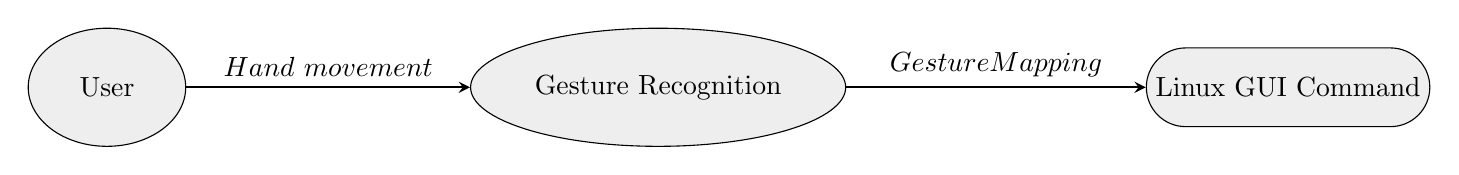
\begin{tikzpicture}[node distance=7cm]
    \node (proc1) [oval2]{User};
    \node (proc2) [oval2, minimum width=10mm,right of = proc1]{Gesture Recognition};
    \node (proc3) [process1,minimum size=10 mm, right of = proc2,xshift= 10 mm]{Linux GUI Command};

    \draw[arrow] (proc1)--(proc2) node[midway,above,rotate=0] {$Hand\ movement$};
    \draw[arrow] (proc2)--(proc3) node[midway,above,rotate=0] {$Gesture Mapping$};
%    \draw [black] ([yshift=0.2cm]proc3.west)--([yshift=0.2cm]proc3.east);

\end{tikzpicture}}
\\
\section{Level 1}
\resizebox{\columnwidth}{!}{
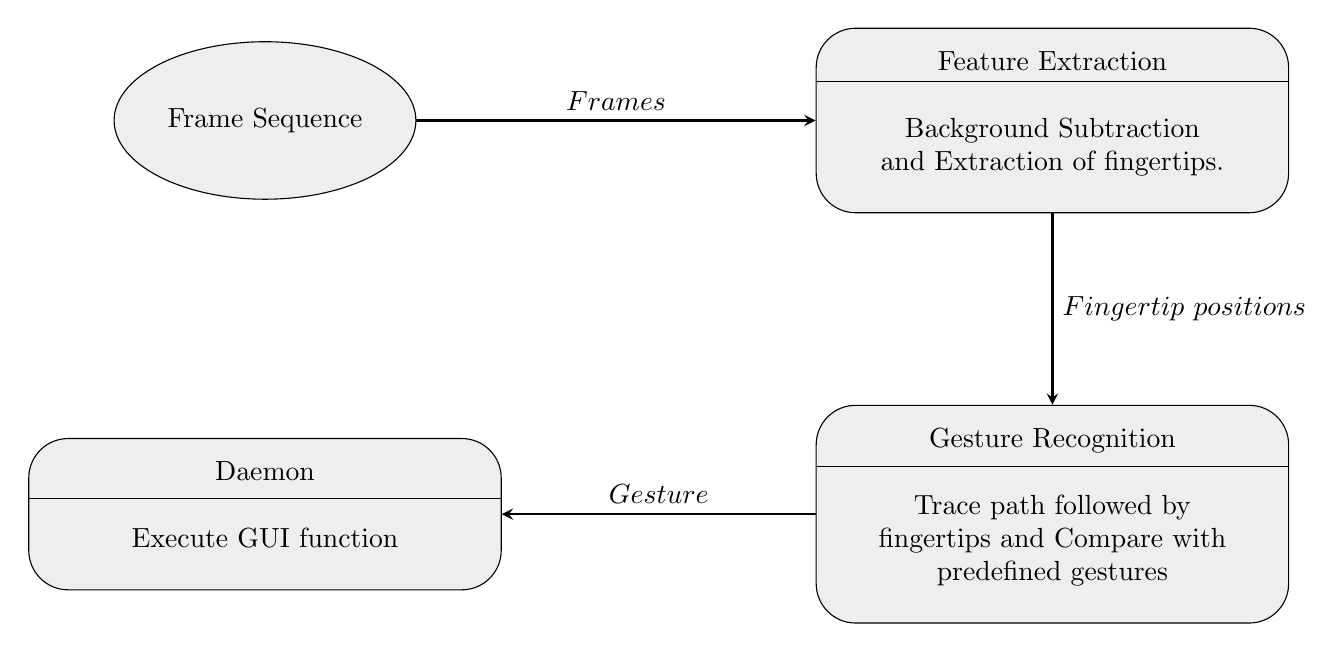
\begin{tikzpicture}[node distance=2cm]
    \node (proc1) [oval]{Frame Sequence};
    \node (proc2) [process1, right of = proc1, xshift=8 cm]{\\Feature Extraction\\\\
    Background Subtraction\\
    and Extraction of fingertips.\\};
    \node (proc3) [process1, below of = proc2, yshift=-3cm]{\\Gesture Recognition\\\\
    Trace path followed by\\
    fingertips and Compare with\\
    predefined gestures\\};
    \node (proc4) [process1, left of = proc3, xshift=-8cm]{\\Daemon\\\\Execute GUI function\\};
    \draw[arrow] (proc1)--(proc2) node[midway,above,rotate=0] {$Frames$};
    \draw[arrow] (proc2)--(proc3) node[midway,right,rotate=0]{$Fingertip\ positions$};
    \draw[arrow] (proc3)--(proc4) node[midway,above,rotate=0] {$Gesture$};
    \draw [black] ([yshift=0.5cm]proc2.west)--([yshift=0.5cm]proc2.east);
    \draw [black] ([yshift=0.6cm]proc3.west)--([yshift=0.6cm]proc3.east);
    \draw [black] ([yshift=0.2cm]proc4.west)--([yshift=0.2cm]proc4.east);
\end{tikzpicture}}

\section{Level 2}
\resizebox{\columnwidth}{!}{
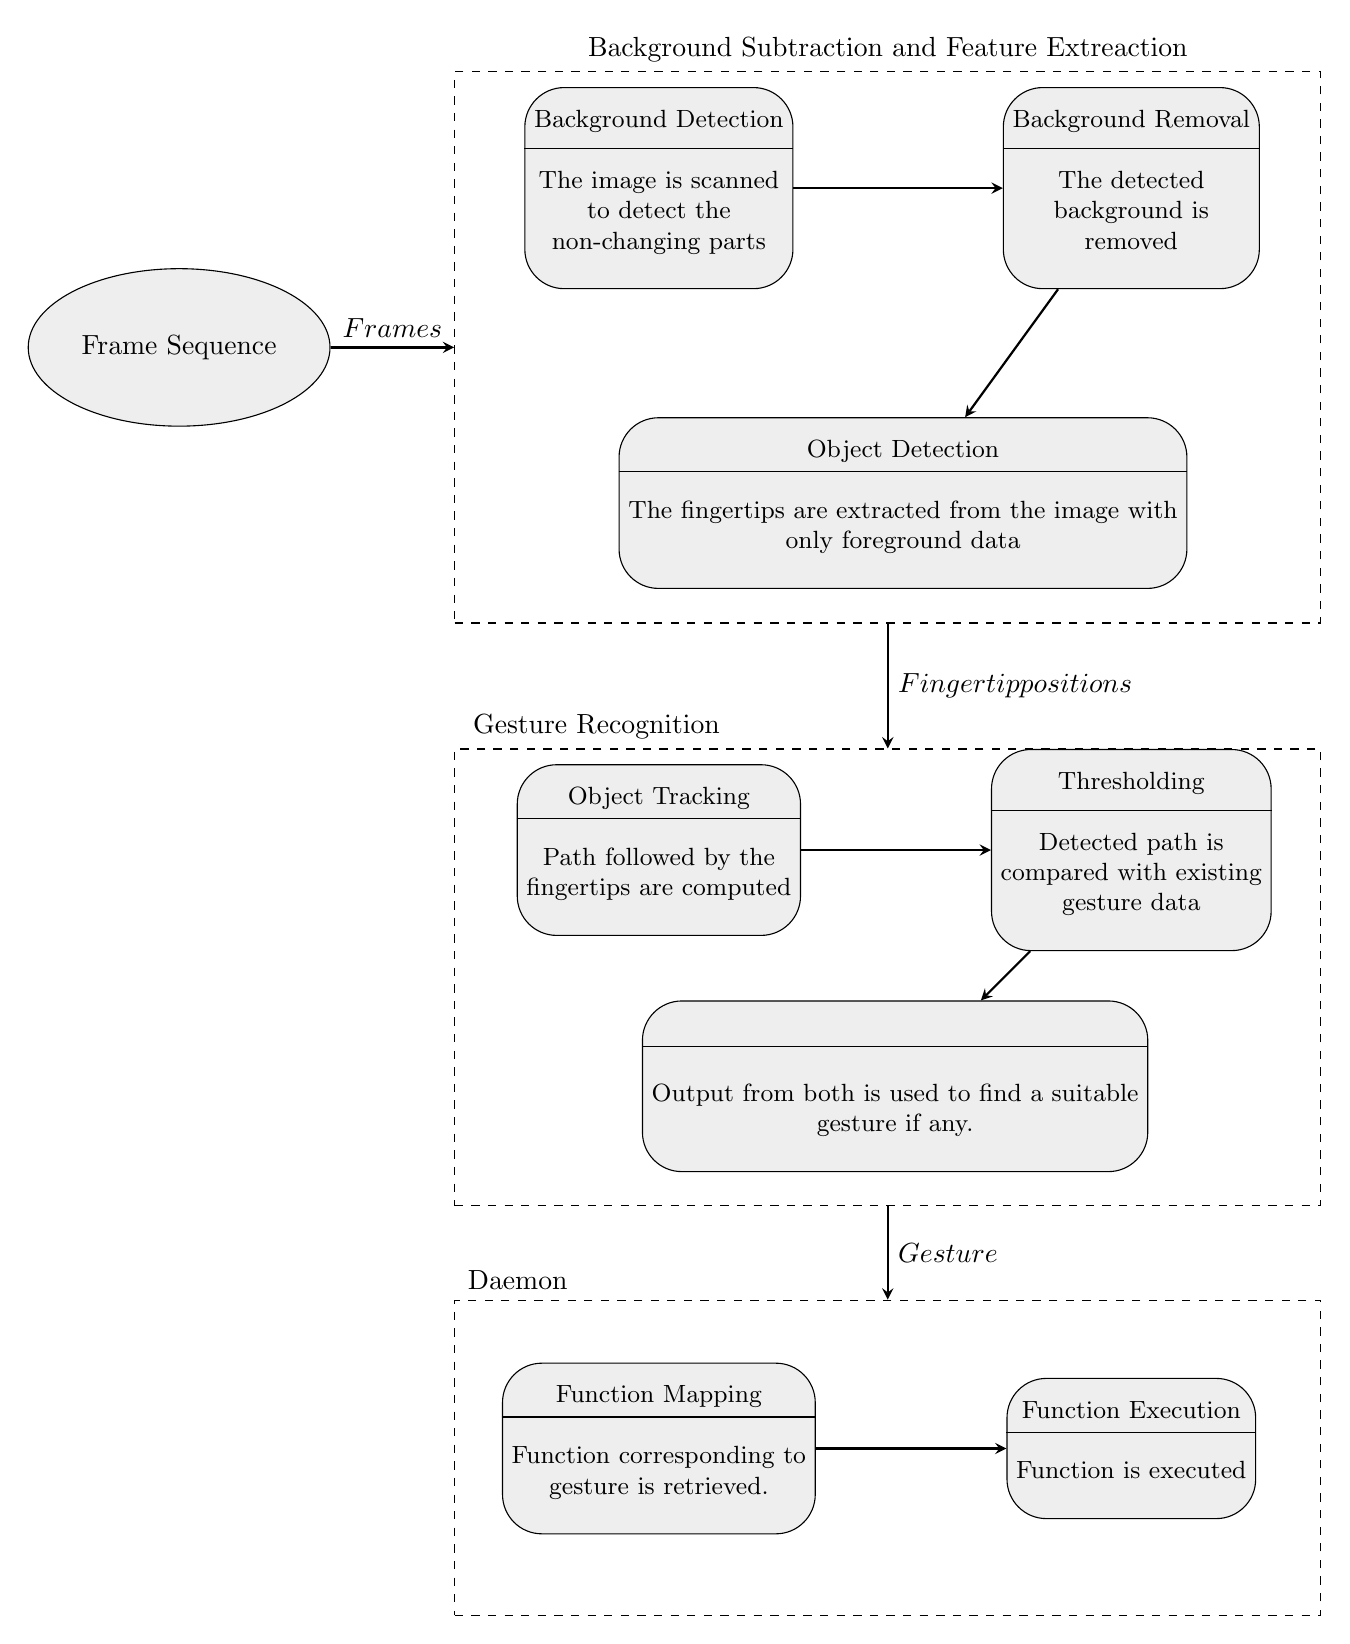
\begin{tikzpicture}[node distance=0cm]
    \node (proc1) [oval]{Frame Sequence};

    \node (over1) [overlay, label=above:Background Subtraction and Feature Extreaction, minimum width = 11cm, minimum height = 7cm, right of = proc1, xshift=9cm]{};

    \node (proc2) [process2, below=of over1.north west, xshift=2.6cm, yshift=-0.2cm]{\\Background Detection\\\\
    The image is scanned\\
    to detect the\\
    non-changing parts\\};


    \node (proc3) [process2, right of = proc2, xshift=6cm]{\\Background Removal\\\\
    The detected\\
    background is\\
    removed\\};

    \node (proc4) [process2, left of = proc3, xshift=-2.9cm, yshift=-4cm]{\\Object Detection\\\\
    The fingertips are extracted from the image with\\
    only foreground data\\};

    \draw [arrow] (proc1)--(over1) node[midway,above,rotate=0] {$Frames$};
    \draw [black] ([yshift=0.5cm]proc2.west)--([yshift=0.5cm]proc2.east);
    \draw [black] ([yshift=0.5cm]proc3.west)--([yshift=0.5cm]proc3.east);
    \draw [black] ([yshift=0.4cm]proc4.west)--([yshift=0.4cm]proc4.east);
    \draw [arrow] (proc2)--(proc3) node[midway, above]{$$};
    \draw [arrow] (proc3)--(proc4) node[midway, above]{$$};
    \node (over2) [overlay, label={[xshift=-3.7cm]Gesture Recognition}, minimum width = 11cm, minimum height = 5.8cm, right of = over1, yshift=-8cm]{};

    \node (proc5) [process2, below=of over2.north west, xshift=2.6cm, yshift=-0.2cm]{\\Object Tracking\\\\
    Path followed by the\\
    fingertips are computed\\};

    \node (proc6) [process2, right of = proc5, xshift=6cm]{\\Thresholding\\\\
    Detected path is\\
    compared with existing\\
    gesture data\\};

    \node (proc7) [process2, left of = proc6, xshift=-3cm, yshift=-3cm]{\\\\\\
    Output from both is used to find a suitable\\
    gesture if any.\\};
    \draw [arrow] (over1)--(over2) node[midway, right]{$Fingertip positions$};
    \draw [black] ([yshift=0.4cm]proc5.west)--([yshift=0.4cm]proc5.east);
    \draw [black] ([yshift=0.5cm]proc6.west)--([yshift=0.5cm]proc6.east);
    \draw [black] ([yshift=0.5cm]proc7.west)--([yshift=0.5cm]proc7.east);
    \draw [arrow] (proc5)--(proc6) node[midway, below]{$$};
    \draw [arrow] (proc6)--(proc7) node[midway, below]{$$};

    \node (over3) [overlay, label={[xshift=-4.7cm]Daemon}, minimum width = 11cm, minimum height = 4cm, right of = over2, yshift=-6.1cm]{};

    \node (proc8) [process2, below=of over3.north west, xshift=2.6cm, yshift=-0.8cm]{\\Function Mapping\\\\
    Function corresponding to\\
    gesture is retrieved.\\};

    \node (proc9) [process2, right of = proc8, xshift=6cm]{\\Function Execution\\\\
    Function is executed\\};
    \draw [arrow] (proc8)--(proc9) node[midway, below]{$$};

    \draw [arrow] (over2)--(over3) node[midway, right]{$Gesture$};

    \draw [black] ([yshift=0.4cm]proc8.west)--([yshift=0.4cm]proc8.east);
    \draw [black] ([yshift=0.2cm]proc9.west)--([yshift=0.2cm]proc9.east);

\end{tikzpicture}}

\chapter{Implementation}
\section{Algorithms}
\subsection{Overall algorithm}
\begin{itemize}
    \item Input: A set of contiguous image frames
    \item Output: The mapped GUI function
    \item Method:
    \begin{enumerate}
        \item Calculate the foreground using MOG2 background subtraction algorithm.
        \item Detect the fingertips using the Convex Hull algorithm.
        \item Track the finger gesture using Continuously Adaptive Mean Shift (CAMshift) algorithm.
        \item Save the above tracked graph to a DetectedGesture object.
        \item Find the closest SavedGesture object and execute the GUI function.
    \end{enumerate}
\end{itemize}
\subsection{Background subtraction}
\begin{enumerate}
    \item Purpose: To find the Region of Interest by subtracting the background from the image frame.
    \item Input: Image frames with foreground and background.
    \item Output: Image frames with only foreground. 
    \item Method:
    \begin{itemize}
        \item Model each background pixel by a mixture of K Gaussian distributions (K = 3 to 5)
        \item Calculate the weights of the mixture which represent the time proportions that those colours stay in the scene.
        \item Remove the colours are which stay longer and more static.
    \end{itemize}
\end{enumerate}
\subsection{Convex Hull}
\begin{itemize}
    \item Purpose: To find the positions of the fingertips in the image frame.
    \item Input: Image frames with background subtracted.
    \item Output: List of Convex Hull peaks
    \item Method:
    \begin{enumerate}
        \item Threshold the image, and retrieve the points in the plane. Let's say there are P points.
        \item Initialize p as leftmost point.
        \item Do following while we don’t come back to the first (or leftmost) point.
        \begin{enumerate}
            \item The next point q is the point such that the triplet (p, q, r) is counterclockwise for any other point r.
            \item next[p] = q (Store q as next of p in the output convex hull).
            \item p = q (Set p as q for next iteration).
        \end{enumerate}
    \end{enumerate}
\end{itemize}
\subsection{CAMShift}
\begin{itemize}
    \item Purpose: To map the positions of the fingertips in the multiple frames to one fluid motion, in the form of lines/curves in a 2D plane.
    \item Input: Sequence of frames with Convex Hull peaks.
    \item Output: 2D plane with a set of lines/curves representing the fluid motion of the fingertips.
    \item Method:
    \begin{enumerate}
        \item Set the calculation region of the probability distribution equal to the whole frame.
        \item Choose the initial location of the two-dimensional mean shift search window.
        \item Calculate the colour probability distribution in the 2D region centred on the search window location in an area slightly larger than the mean shift window size.
        \item Perform the search of the maximum density probability using the mean shift parameter for convergence or for setting the number of iterations. Store the zero moment (area or size) and middle position.
        \item For the next image frame, place the search window in the middle position fixed in step 4, and set the window size in conformity to the last moment. Go to step 3. 
    \end{enumerate}
\end{itemize}
\subsection{Brute Force Matching}
\begin{itemize}
    \item Purpose: To match the DetectedGesture to a SavedGesture, and execute the corresponding GUI function.
    \item Input: The feature objects encoded in the SavedFeature and DetectedFeature objects.
    \item Output: A quantity representing the closeness of the two gestures.
    \item Method:
    \begin{enumerate}
        \item For a given keypoint K1 from the first set, take every keypoint in the second set and calculate the distance.
        \item Distance formula used is Euclidean distance. The sum of the distances on each dimension is finally used to calculate the returned quantity.
        \item cv2.NORM2 can be used to find the BFMatch value between two sets (of points)
        \item The Euclidean Distance sum is normalized and returned.
    \end{enumerate}
\end{itemize}
\section{Development Tools}
\subsection{Sublime Text}
Sublime Text is a proprietary cross-platform source code editor with a Python application program-
ming interface (API). It natively supports many programming languages and markup languages,
and functions can be added by users with plugins, typically community-built and maintained under
free-software licenses.
Some of the features of Sublime Text are
\begin{itemize}
\item ”Goto Anything,”quick navigation to files, symbols, or lines
\item ”Command palette” uses adaptive matching for quick keyboard invocation of arbitrary com-
mands
\item Simultaneous editing: simultaneously make the same interactive changes to multiple selected
areas
\item Python-based plugin API
\item Project-specific preferences
\item Extensive customizability via JSON settings files, including project-specific and platform-
specific settings
\item Cross platform (Windows, macOS, and Linux)

\end{itemize}

\chapter{Testing}
Software testing is an investigation conducted to provide stakeholders with information about
the quality of the product or service under test. Software testing can also provide an objective,
independent view of the software to allow the business to appreciate and understand the risks of
software implementation. Test techniques include the process of executing a program or application
with the intent of finding software bugs, and to verify that the software product is fit for use.
Software testing involves the execution of a software component or system component to evaluate
one or more properties of interest. In general, these properties indicate the extent to which the
component or system under test
\begin{itemize}
    \item Meets the requirements that guided its design and development,
    \item Responds correctly to all kinds of inputs
    \item Performs its functions within an acceptable time
\item Is sufficiently usable
\item Can be installed and run in its intended environments, and
\item Achieves the general result its stakeholders desire.
\end{itemize}
\section{Testing Methodologies}
Software testing methodology is for making sure that software products/systems developed have
been successfully tested to meet their specified requirements and can successfully operate in all the
anticipated environments with required usability and security.
Software testing methods are traditionally divided into white and black-box testing. These two
approaches are used to describe the point of view that a test engineer takes when designing test
cases.
White-box testing by seeing the source code tests internal structures or workings of a program, as
opposed to the functionality exposed to the end-user. In white-box testing an internal perspective
of the system, as well as programming skills, are used to design test cases. The tester chooses in-
puts to exercise paths through the code and determine the appropriate outputs. This is analogous
to testing nodes in a circuit. While white-box testing can be applied at the unit, integration and system levels of the software testing process, it is usually done at the unit level.
Black-box testing treats the software as a black-box , examining functionality without any knowl-
edge of internal implementation, without seeing the source code. The testers are only aware of
what the software is supposed to do, not how it does it. Here the black-box testing is used for the
system. The testing methods applied were:

\begin{itemize}
    \item Unit Testing \\
Unit testing is a software development process in which the smallest testable parts of an
application, called units, are individually and independently scrutinized for proper operation.
    \item Integration Testing \\
    Integration testing is the phase in software testing in which individual software modules are
    combined and tested as a group. It occurs after unit testing.
    \item System Testing \\
    System testing of software or hardware is testing conducted on a complete, integrated system
    to evaluate the system’s compliance with its specified requirements. System testing falls
    within the scope of black-box testing, and as such, should require no knowledge of the inner
    design of the code or logic.
\end{itemize}
\section{Unit Testing}
In the unit testing phase, the Background Subtraction Module, Feature Extraction, Finger-tip Tracking, Gesture Recognition
and Gesture mapping were separately tested.

\subsection{Background Subtraction Module}

The images from the camera feed is provided to the Background Subtraction
module in RGB colour space. The output images were in HSV filtered with Colour Ranges as expected.

\begin{figure}[h]
    \includegraphics[width=15cm]{backgroundtesting.png}
    \caption{Background Subtraction Module}
\end{figure}

\subsection{Feature Extraction}

The output from the background subtraction module is fed into the feature Extraction
module. This module computes the convex hull and finds the separate shapes and finds the centroids of 
each hull.

\begin{figure}[h]
    \includegraphics[width=15cm]{featuretest.png}
    
    \includegraphics[width=15cm]{featuretest2.png}
    \caption{Feature Extraction Module}
\end{figure}

\subsection{FingerTip Tracking and Gesture Recognition}

The Finger tip tracking module tracks the centroids movement over multiple frames and the Gesture Recognition Module recognizes the gesture.

\begin{figure}[H]
    \includegraphics[width=15cm]{gesture.png}
    
    \caption{Finger Tip Tracking and Gesture Recognition}
\end{figure}



\section{Integration Testing}

Different modules were combined and was tested to see if the modules interact properly and produce
correct output. The Background Subtraction Module provided its output to the feature extraction module
which then finds the convex hulls. The output is passed to the finger-tip tracking module which tracks the 
direction and number of fingers. The output is successfully passed to the Gesture Recognition module which allots the gesture.
Finally the output is passed to the Gesture Map module which executes the gesture in the Linux GUI.

\section{System Testing}

After the integration testing, we do the system testing. In system testing the whole modules are
connected in order; the background subtraction module is integrated with the feature extraction module,the
feature extraction module is integrated with the fingertip tracking and also the gesture recognition
module and gesture mapping module. The whole system is inte-
grated.



\chapter{Graphical User Interface}
\section{GUI Overview}
\section{Main GUI Components}

\chapter{Results}
Include screenshots of the project.

\chapter{Conclusion}

\chapter{Future Scope}

\chapter{Publication}
   
\begin{thebibliography}{999}
\addcontentsline{toc}{chapter}{References}
\bibitem{}


\end{thebibliography}

\end{document}
